\documentclass[11pt]{amsart}
\usepackage{amsmath}
\usepackage{amssymb}
\usepackage{tikz}
\tikzset{vtx/.style={inner sep=1.7pt, outer sep=0pt, circle, fill,draw}}

\begin{document}

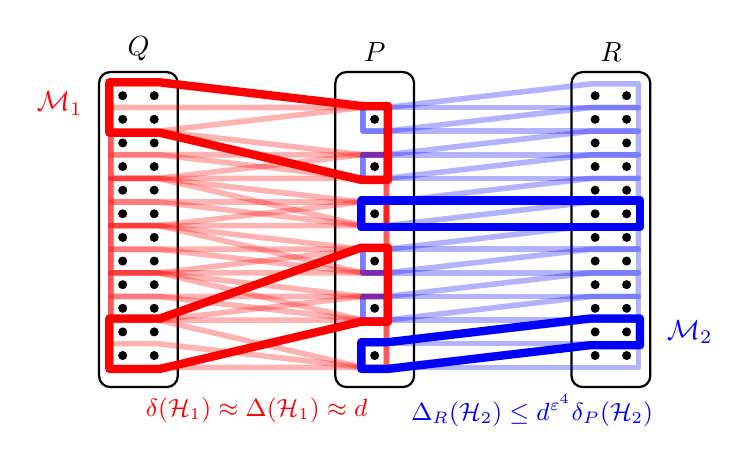
\begin{tikzpicture}
	\def \px {0};
	\def \qx {-3};
	\def \rx {3};			

	%P,Q,R
	\node at (\px, 0) [draw,rectangle,minimum width=1cm,minimum height=4cm,rounded corners,thick,label=$P$] {};
	\node at (\qx, 0) [draw,rectangle,minimum width=1cm,minimum height=4cm,rounded corners,thick,label=$Q$] {};
	\node at (\rx, 0) [draw,rectangle,minimum width=1cm,minimum height=4cm,rounded corners,thick,label=$R$] {};

	% List of y coords
	\def \ylist {1.7, 1.4, 1.1, 0.8, 0.5, 0.2, -0.1, -0.4, -0.7, -1, -1.3, -1.6};
	\def \halfylistl {1.4, 0.8, 0.2, -0.4, -1, -1.6};
	\def \halfylists {1.4, 0.8, 0.2, -0.4, -1};

	% P vertices
	\foreach \y in \halfylistl \node at (0, \y) [vtx,inner sep=1pt] {};

	% Q vertices
	\foreach \x in {\qx-0.2, \qx+0.2} \foreach \y in \ylist \node at (\x, \y) [vtx,inner sep=1pt] {};

	% R vertices
	\foreach \x in {\rx-0.2,\rx+0.2} \foreach \y in \ylist \node at (\x, \y) [vtx,inner sep=1pt] {};			

	\def \edgesep {0.15};
	\def \pheight {0.6};
	\foreach \py in \halfylists {\foreach \qy in {\py + 0.3, \py, \py - 0.3} {
		\pgfmathrandominteger{\r}{3}{12}
		\draw[color=red, opacity=0.3, line cap=round, line join=round, line width=2pt] (\px+\edgesep, \py+\edgesep) -- (\px-\edgesep, \py+\edgesep) -- (\qx+0.1+\edgesep, \qy+\edgesep) -- (\qx-0.2-\edgesep, \qy+\edgesep) -- (\qx-0.2-\edgesep, \qy-0.3-\edgesep) -- (\qx+0.1+\edgesep, \qy-0.3-\edgesep) -- (\px-\edgesep, \py-\pheight-\edgesep) -- (\px+\edgesep, \py-\pheight-\edgesep) -- (\px+\edgesep, \py+\edgesep);
	}};

	\def \edgesep {0.15};
	\def \pheight {0};
	\foreach \py in \halfylistl {\foreach \qy in {\py + 0.3, \py} {
		\pgfmathrandominteger{\r}{3}{12}
		\draw[color=blue, opacity=0.3, line cap=round, line join=round, line width=2pt] (\px-\edgesep, \py+\edgesep) -- (\px+\edgesep, \py+\edgesep) -- (\rx-0.1-\edgesep, \qy+\edgesep) -- (\rx+0.2+\edgesep, \qy+\edgesep) -- (\rx+0.2+\edgesep, \qy-\edgesep) -- (\rx-0.1-\edgesep, \qy-\edgesep) -- (\px+\edgesep, \py-\pheight-\edgesep) -- (\px-\edgesep, \py-\pheight-\edgesep) -- (\px-\edgesep, \py+\edgesep);
	}};

	\def \edgesep {0.17};
	\def \py {1.4};
	\def \qy {1.7};
	\def \pheight {0.6};
	\draw[color=red, line cap=round, line join=round, line width=3pt] (\px+\edgesep, \py+\edgesep) -- (\px-\edgesep, \py+\edgesep) -- (\qx+0.1+\edgesep, \qy+\edgesep) -- (\qx-0.2-\edgesep, \qy+\edgesep) -- (\qx-0.2-\edgesep, \qy-0.3-\edgesep) -- (\qx+0.1+\edgesep, \qy-0.3-\edgesep) -- (\px-\edgesep, \py-\pheight-\edgesep) -- (\px+\edgesep, \py-\pheight-\edgesep) -- (\px+\edgesep, \py+\edgesep);
	\def \py {-0.4}
	\def \qy {-1.3};
	\draw[color=red, line cap=round, line join=round, line width=3pt] (\px+\edgesep, \py+\edgesep) -- (\px-\edgesep, \py+\edgesep) -- (\qx+0.1+\edgesep, \qy+\edgesep) -- (\qx-0.2-\edgesep, \qy+\edgesep) -- (\qx-0.2-\edgesep, \qy-0.3-\edgesep) -- (\qx+0.1+\edgesep, \qy-0.3-\edgesep) -- (\px-\edgesep, \py-\pheight-\edgesep) -- (\px+\edgesep, \py-\pheight-\edgesep) -- (\px+\edgesep, \py+\edgesep);

	\def \edgesep {0.17};
	\def \py {0.2};
	\def \qy {0.2};
	\def \pheight {0};
	\draw[color=blue, line cap=round, line join=round, line width=3pt] (\px-\edgesep, \py+\edgesep) -- (\px+\edgesep, \py+\edgesep) -- (\rx-0.1-\edgesep, \qy+\edgesep) -- (\rx+0.2+\edgesep, \qy+\edgesep) -- (\rx+0.2+\edgesep, \qy-\edgesep) -- (\rx-0.1-\edgesep, \qy-\edgesep) -- (\px+\edgesep, \py-\pheight-\edgesep) -- (\px-\edgesep, \py-\pheight-\edgesep) -- (\px-\edgesep, \py+\edgesep);
	\def \py {-1.6};
	\def \qy {-1.3};
	\draw[color=blue, line cap=round, line join=round, line width=3pt] (\px-\edgesep, \py+\edgesep) -- (\px+\edgesep, \py+\edgesep) -- (\rx-0.1-\edgesep, \qy+\edgesep) -- (\rx+0.2+\edgesep, \qy+\edgesep) -- (\rx+0.2+\edgesep, \qy-\edgesep) -- (\rx-0.1-\edgesep, \qy-\edgesep) -- (\px+\edgesep, \py-\pheight-\edgesep) -- (\px-\edgesep, \py-\pheight-\edgesep) -- (\px-\edgesep, \py+\edgesep);

	% Matching names
	\node at (\qx - 1, 1.6) [red] {$\mathcal{M}_1$};
	\node at (\rx + 1, -1.3) [blue] {$\mathcal{M}_2$};

	% Degrees
	\node at (0.5*\qx + 0.5*\px, -2.3) [red] {\small $\delta(\mathcal{H}_1) \approx \Delta(\mathcal{H}_1) \approx d$};
	\node at (\rx-1, -2.3) [blue] {\small $\Delta_R(\mathcal{H}_2) \le d^{\varepsilon^4} \delta_{P}(\mathcal{H}_2)$};
\end{tikzpicture}

\end{document}